\documentclass[border=0pt]{standalone}

\usepackage{xcolor}
\usepackage{tikz}
\usepackage[utf8]{inputenc}
\usepackage[T1]{fontenc}
\usepackage{lmodern}
\usepackage{amsmath}
\usetikzlibrary{arrows.meta}

% ── Colores Springer ───────────────────────────────────────────────
\definecolor{springerred}{RGB}{192, 57, 43}
\definecolor{creamBG}{RGB}{245, 240, 232}
\definecolor{darktext}{RGB}{26, 16, 8}
\definecolor{mutedtext}{RGB}{90, 74, 58}
\definecolor{lightborder}{RGB}{200, 191, 175}
\definecolor{bottombg}{RGB}{237, 232, 220}
\definecolor{nightblue}{RGB}{15, 15, 42}
\definecolor{gridblue}{RGB}{42, 48, 96}
\definecolor{axisblue}{RGB}{74, 80, 144}
\definecolor{vecred}{RGB}{231, 76, 60}
\definecolor{vecblue}{RGB}{52, 152, 219}
\definecolor{vecgreen}{RGB}{39, 174, 96}

\begin{document}

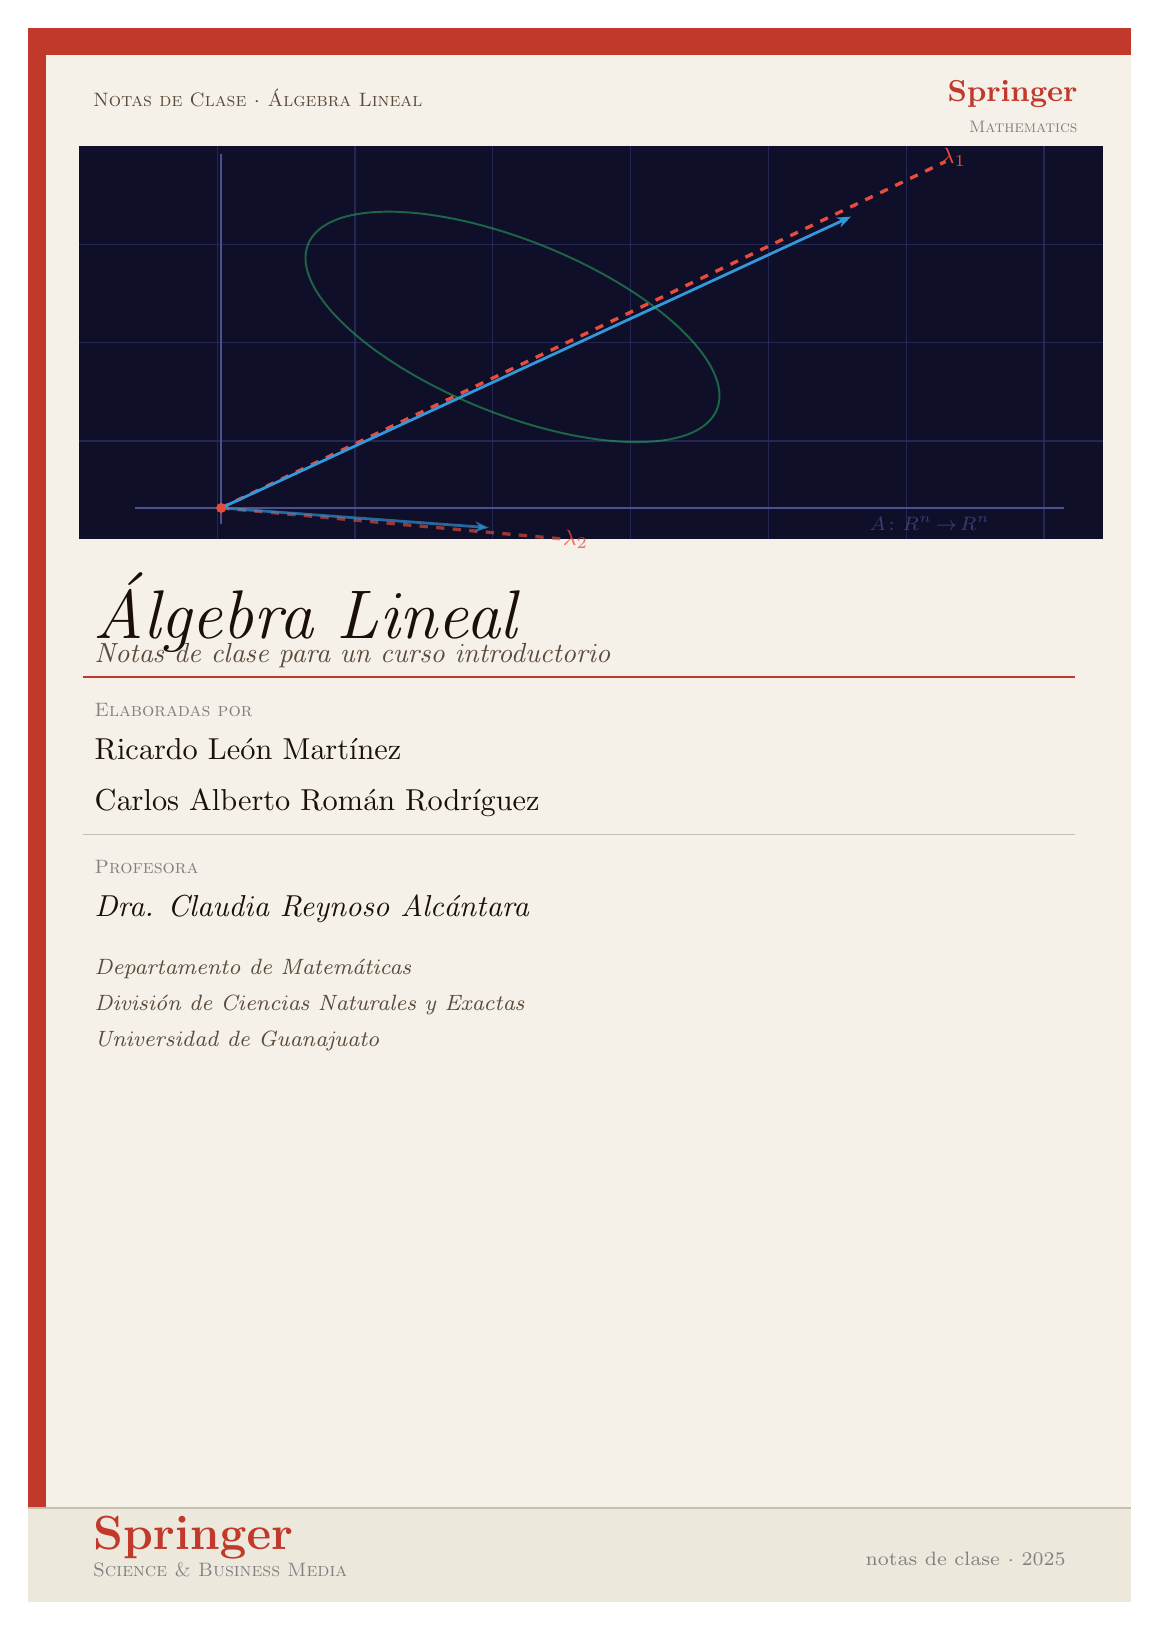
\begin{tikzpicture}

  % ── Dimensiones de la portada (14cm x 20cm) ──────────────────────
  \def\W{14}   % ancho total en cm
  \def\H{20}   % alto total en cm

  % ── Fondo crema ──────────────────────────────────────────────────
  \fill[creamBG] (0,0) rectangle (\W,\H);

  % ── Franja roja superior ─────────────────────────────────────────
  \fill[springerred] (0,\H) rectangle (\W,{\H-0.35});

  % ── Lomo rojo izquierdo ──────────────────────────────────────────
  \fill[springerred] (0,0) rectangle (0.22,\H);

  % ── Barra inferior ───────────────────────────────────────────────
  \fill[bottombg] (0,0) rectangle (\W,1.2);
  \draw[lightborder, line width=0.4pt] (0,1.2) -- (\W,1.2);

  % ── Serie (arriba izquierda) ──────────────────────────────────────
  \node[anchor=north west, text=mutedtext,
        font=\fontsize{7}{9}\selectfont\scshape]
    at (0.7,{\H-0.65})
    {Notas de Clase $\cdot$ Álgebra Lineal};

  % ── Logo Springer (arriba derecha) ───────────────────────────────
  \node[anchor=north east]
    at ({\W-0.55},{\H-0.55}) {%
      \begin{minipage}{3cm}\raggedleft
        {\color{springerred}\fontsize{11}{13}\selectfont\textbf{Springer}}\\[-1pt]
        {\color{gray}\fontsize{6}{7}\selectfont\scshape Mathematics}
      \end{minipage}};

  % ── Ilustración matemática ────────────────────────────────────────
  % Recuadro: de x=0.65 a x=13.65, de y=13.5 a y=18.5  (5cm alto, 13cm ancho)
  \begin{scope}[shift={(0.65,13.5)}, x=1cm, y=1cm]
    \def\iW{13.0}
    \def\iH{5.0}

    \fill[nightblue] (0,0) rectangle (\iW,\iH);

    % Grid
    \foreach \xi in {1.75, 3.5, 5.25, 7.0, 8.75, 10.5, 12.25}{
      \draw[gridblue, line width=0.4pt, opacity=0.75] (\xi,0) -- (\xi,\iH);
    }
    \foreach \yi in {1.25, 2.5, 3.75}{
      \draw[gridblue, line width=0.4pt, opacity=0.75] (0,\yi) -- (\iW,\yi);
    }

    % Ejes
    \draw[axisblue, line width=0.8pt] (0.7,0.4) -- (12.5,0.4);
    \draw[axisblue, line width=0.8pt] (1.8,0.2) -- (1.8,4.9);

    % Vectores propios (rojo punteado)
    \draw[vecred, line width=1.2pt, dashed] (1.8,0.4) -- (11.0,4.8);
    \draw[vecred, line width=1.2pt, dashed, opacity=0.65] (1.8,0.4) -- (6.2,0.0);

    % Vectores transformados (azul con flecha)
    \draw[vecblue, line width=1.0pt, -{Stealth[length=5pt]}]
      (1.8,0.4) -- (9.8,4.1);
    \draw[vecblue, line width=1.0pt, -{Stealth[length=5pt]}, opacity=0.65]
      (1.8,0.4) -- (5.2,0.15);

    % Elipse
    \draw[vecgreen, line width=0.7pt, opacity=0.55,
          rotate around={-22:(5.5,2.7)}]
      (5.5,2.7) ellipse (2.8cm and 1.1cm);

    % Etiquetas
    \node[vecred, font=\fontsize{8}{9}\selectfont\itshape] at (11.1,4.85) {$\lambda_1$};
    \node[vecred, font=\fontsize{8}{9}\selectfont\itshape, opacity=0.75]
      at (6.3,0.0) {$\lambda_2$};
    \node[axisblue, font=\fontsize{7}{8}\selectfont\ttfamily, opacity=0.7]
      at (10.8,0.2) {$A\colon\mathbb{R}^n\!\to\!\mathbb{R}^n$};

    % Origen
    \fill[vecred] (1.8,0.4) circle (1.8pt);
  \end{scope}

  % ── Título principal ──────────────────────────────────────────────
  \node[anchor=north west, text=darktext,
        font=\fontsize{30}{34}\selectfont\itshape]
    at (0.7,13.2)
    {Álgebra Lineal};

  % ── Subtítulo ─────────────────────────────────────────────────────
  \node[anchor=north west, text=mutedtext,
        font=\fontsize{10}{13}\selectfont\itshape]
    at (0.72,12.3)
    {Notas de clase para un curso introductorio};

  % ── Línea divisoria roja ──────────────────────────────────────────
  \draw[springerred, line width=0.7pt] (0.7,11.75) -- (13.3,11.75);

  % ── Elaboradas por ───────────────────────────────────────────────
  \node[anchor=north west, text=gray,
        font=\fontsize{7}{9}\selectfont\scshape]
    at (0.72,11.55)
    {Elaboradas por};

  % ── Autores ───────────────────────────────────────────────────────
  \node[anchor=north west, text=darktext,
        font=\fontsize{11}{15}\selectfont]
    at (0.72,11.1)
    {Ricardo León Martínez};

  \node[anchor=north west, text=darktext,
        font=\fontsize{11}{15}\selectfont]
    at (0.72,10.45)
    {Carlos Alberto Román Rodríguez};

  % ── Línea fina ────────────────────────────────────────────────────
  \draw[lightborder, line width=0.4pt] (0.7,9.75) -- (13.3,9.75);

  % ── Profesora ─────────────────────────────────────────────────────
  \node[anchor=north west, text=gray,
        font=\fontsize{7}{9}\selectfont\scshape]
    at (0.72,9.55)
    {Profesora};

  \node[anchor=north west, text=darktext,
        font=\fontsize{11}{14}\selectfont\itshape]
    at (0.72,9.1)
    {Dra. Claudia Reynoso Alcántara};

  % ── Institución ───────────────────────────────────────────────────
  \node[anchor=north west, text=mutedtext,
        font=\fontsize{8.5}{13}\selectfont\itshape, align=left]
    at (0.72,8.3)
    {Departamento de Matemáticas\\
     División de Ciencias Naturales y Exactas\\
     Universidad de Guanajuato};

  % ── Logo Springer abajo izquierda ────────────────────────────────
  \node[anchor=south west]
    at (0.7,0.2) {%
      \begin{minipage}{5cm}
        {\color{springerred}\fontsize{16}{18}\selectfont\textbf{Springer}}\\[-2pt]
        {\color{gray}\fontsize{7}{8}\selectfont\scshape Science \& Business Media}
      \end{minipage}};

  % ── Año abajo derecha ─────────────────────────────────────────────
  \node[anchor=south east, text=gray,
        font=\fontsize{7}{9}\selectfont]
    at ({\W-0.7},0.35)
    {notas de clase $\cdot$ 2025};

\end{tikzpicture}

\end{document}
